\scanpage{4}
\begingroup\ttfamily

% letterhead
\noindent
\begin{minipage}[t]{.48\linewidth}\centering
U N I V E R S I T E\\
DES SCIENCES ET TECHNIQUES\\
DU LANGUEDOC\\
{\footnotesize $\frown\frown\frown\frown\frown\frown\frown\frown\frown\frown\frown\frown$}\\[.6em]
Service de la Scolarité\\
JP/GJ\\[.5em]
\uline{Diffusion} : Liste A\\
N°: 2418
\end{minipage}\hfill
\begin{minipage}[t]{.49\linewidth}\raggedleft
MONTPELLIER, le 19 AVRIL 1977\\
\end{minipage}

\begin{center}
\uline{AVIS DE SOUTENANCE D'UNE THESE DE DOCTORAT DE}\\[.5em]
\uline{SPECIALITE : SCIENCES DE LA TERRE mention GEOLOGIE APPLIQUEE}
\end{center}

\uline{Nom et prénom du candidat} : BAYER Michel

\uline{Titre de la thèse} : Etude gravimétrique de la Corse.

\uline{Date, heure et lieu de soutenance prévus} : 25 AVRIL 1977 à 14 h. 30

\hspace*{3em}Salle de cours n° 10 - U.S.T.L.

\uline{Nom du Directeur de thèse} : M. LOUIS Pierre

\uline{Désignation du laboratoire où la thèse est préparée} :

\hspace*{3em}Laboratoire de Géophysique

\uline{Analyse de l'ouvrage} : Afin de terminer le levé gravimétrique de la Corse, 270 mesures ont été effectuées. L'ensemble des données (720 stations) a été traité (cartes de l'anomalie de Bouguer, dérivées, régionales et résiduelles) puis interprété, en tenant compte de la géologie et de l'aéromagnétisme. Des hypothèses sont proposées, en particulier pour la structure profonde de la Corse et des régions avoisinantes (bassin Algéro-provençal).

\uline{Durée approximative des recherches ayant abouti à la thèse} : Deux ans

\uline{Composition du jury proposé} :

\begin{center}
\begin{tabular}{r@{\quad}l}
MM. : & P. LOUIS\\
      & M. MATTAUER\\
      & R. NEUMANN\\
Mlle  & F. RIMBERT\\
M.    & J. ORSINI
\end{tabular}
\end{center}

\noindent\hfill\begin{minipage}{.49\linewidth}\centering
Le Secrétaire Général,\\[.7em]
\figure{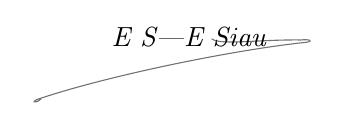
\begin{tikzpicture}[x=.70cm,y=.70cm,line cap=round]
\draw[thin,black!55] (-2.22,-.72) .. controls (-2.32,-.82) and (-2.45,-.77) .. (-2.20,-.70)
 .. controls (-.96,-.29) and (1.27,.17) .. (2.61,.31)
 .. controls (2.72,.33) and (2.66,.37) .. (2.50,.35)
 .. controls (1.70,.36) and (1.04,.25) .. (.88,.37);
\node[anchor=base,inner sep=0pt] at (.46,.23) {\normalfont\itshape\handwritten{\unsure{E S|E Siau}}};
\end{tikzpicture}}
\uline{E. SIAU}\\
\end{minipage}
\endgroup
% archive sheet number: 3
